\section{Excitons and the Bethe--Salpeter equation}\label{sec:4.9}

The measured absorption spectrum of silicon has a peak of height 36 at \SI{3.42}{eV}, and every approximation of \cref{sec:4.6} leaves only a shoulder of 13 to 15 in its place (\cref{fig:4-si-approx}). The bubble, the local fields and the adiabatic kernel all treat the electron lifted across the gap and the hole it leaves behind as independent. In fact the two carry opposite charges and attract, and the other electrons screen their attraction without cancelling it. In GaAs the attraction binds them into a hydrogen-like state \SI{4.2}{meV} below the gap, which shows up as a sharp line at the absorption edge~\cite{sell1972resolved}, and in silicon the bound pair lies \SI{14.7}{meV} below the indirect gap~\cite{shaklee1970valley}. Such correlated electron--hole pairs, bound or not, are excitons. For dark matter they matter exactly where light particles probe the target: in the first eV above the gap, where the loss function is smallest and the attraction moves spectral weight downward and adds lines below the continuum.

\subsection{The electron--hole Hamiltonian}

In the bubble of \cref{sec:4.8} one density vertex creates a pair, an electron in $(c,\vect{k}+\vect{q})$ and a hole in $(v,\vect{k})$, and the other vertex destroys it; such a pair is a transition, labeled $cv\vect{k}$ at fixed $\vect{q}$. Between the two vertices the pair propagates freely, and in an insulator at $T = 0$ each transition is an eigenstate of the problem with energy $\varepsilon_{c,\vect{k}+\vect{q}} - \varepsilon_{v\vect{k}}$. The ladder of \cref{fig:4-diagrams}(d) lets the electron and the hole interact any number of times on the way, and \cref{app:D.12} sums it with the rules of \cref{app:D.11}. The two first-order insertions of \cref{sec:4.8} become two kernels, and with a statically screened interaction line the sum closes as a matrix equation in the space of transitions, which is an eigenvalue problem.
\begin{keyresult}[Bethe--Salpeter equation in the transition basis]
At momentum transfer $\vect{q}$, the exciton energies $E_\lambda(\vect{q})$ and envelopes $A^\lambda_{cv\vect{k}}(\vect{q})$ solve
\begin{equation}
  \begin{gathered}
  \sum_{c'v'\vect{k}'}H^{\mathrm{exc}}_{cv\vect{k},c'v'\vect{k}'}\,A^\lambda_{c'v'\vect{k}'} = E_\lambda\,A^\lambda_{cv\vect{k}}, \\
  H^{\mathrm{exc}}_{cv\vect{k},c'v'\vect{k}'} = \bigl(\varepsilon_{c,\vect{k}+\vect{q}} - \varepsilon_{v\vect{k}}\bigr)\delta_{cc'}\delta_{vv'}\delta_{\vect{k}\vect{k}'} + g_{\mathrm{deg}}K^{\mathrm{x}}_{cv\vect{k},c'v'\vect{k}'} - K^{\mathrm{d}}_{cv\vect{k},c'v'\vect{k}'} ,
  \end{gathered}
  \label{eq:4.9-bse}
\end{equation}
normalized to $\sum_{cv\vect{k}}|A^\lambda_{cv\vect{k}}|^2 = 1$, with $g_{\mathrm{deg}} = 2$ for the spin singlets that the density creates. The exchange and direct kernels are
\begin{equation}
  \begin{aligned}
  K^{\mathrm{x}}_{cv\vect{k},c'v'\vect{k}'} &= \frac1\Vol\sum_{\vect{G}\ne0}v_{\mathrm{C}}(|\vect{q}+\vect{G}|)\,\rho_{cv}(\vect{k},\vect{q}+\vect{G})\,\rho_{c'v'}(\vect{k}',\vect{q}+\vect{G})^* ,\\
  K^{\mathrm{d}}_{cv\vect{k},c'v'\vect{k}'} &= \frac1\Vol\sum_{\vect{G}\vect{G}'}\rho_{cc'}(\vect{k}'+\vect{q},\vect{p}+\vect{G})\,W^{\mathrm{scr}}_{\vect{G}\vect{G}'}(\vect{p},\omega = 0)\,\rho_{vv'}(\vect{k}',\vect{p}+\vect{G}')^*, \quad \vect{p} = \vect{k} - \vect{k}' ,
  \end{aligned}
  \label{eq:4.9-kernels}
\end{equation}
with the density vertices of \cref{eq:3.2-rho}, the screened interaction $W^{\mathrm{scr}}_{\vect{G}\vect{G}'} = (\varepsilon^{-1})_{\vect{G}\vect{G}'}v_{\mathrm{C}}(|\vect{p}+\vect{G}'|)$ of \cref{eq:4.8-W}, and quasiparticle band energies.
\end{keyresult}
\Cref{eq:4.9-bse} is \cref{eq:E.6-Hexc} at finite $\vect{q}$. The exchange kernel is the one of \cref{sec:4.6,sec:4.8}, the Coulomb interaction without its $\vect{G} = 0$ term. For a momentum transfer beyond the first zone, $\vect{q} = \vect{q}_r + \vect{G}_q$ in the unreduced indexing of \cref{sec:4.4}, the kernels are written with $\vect{q}_r$ in place of $\vect{q}$, and the omitted term of $K^{\mathrm{x}}$ is then the one at $\vect{G} = \vect{G}_q$.

Each piece of $H^{\mathrm{exc}}$ has a plain meaning. The diagonal is the energy of the free pair. It must be a quasiparticle energy (\cref{sec:4.7}), because the self-energy insertions of the ladder are summed into the propagators, and with Kohn--Sham bands a scissor (\cref{eq:3.4-scissor}) takes their place. The direct kernel is the Coulomb interaction between the electron and the hole, screened by all the other electrons. The electron scatters from $(c,\vect{k}+\vect{q})$ to $(c',\vect{k}'+\vect{q})$ and the hole from $(v,\vect{k})$ to $(v',\vect{k}')$, so the pair keeps its total momentum $\vect{q}$ and its constituents exchange $\vect{p}$. Its diagonal element is the Coulomb energy of two positive densities, $|\psi_{c,\vect{k}+\vect{q}}|^2$ and $|\psi_{v\vect{k}}|^2$. Since that energy is positive, $-K^{\mathrm{d}}$ lowers the pair energy: it is the attraction. At large separation the screened interaction of two charges in an insulator is $e^2/(4\pi\varepsilon_\infty r)$, and this long-range tail is what binds the pairs of the next subsection. The exchange kernel describes something else. The pair annihilates at one point and a pair is re-created at another, and the Coulomb line between them is the microscopic Hartree potential of the induced density. It is the local-field kernel of \cref{sec:4.6}, positive on the diagonal and repulsive. The long-range term $\vect{G} = 0$ is left out because it is the macroscopic field, which the definition of $\varepsilon_{\mathrm{mac}}$ already treats on its own (\cref{eq:D.12-epsmac}); added back, it yields the full density response (\cref{app:D.12}). Exchange is also what distinguishes the spin states. The density vertex couples to both spins alike, so $K^{\mathrm{x}}$ couples a transition of either spin to one of either spin and appears with $g_{\mathrm{deg}}$ in the singlet, while the triplet feels only $-K^{\mathrm{d}}$ and is not excited by a density coupling at all.

Behind \cref{eq:4.9-bse} stand a kernel without the change of the screening, a static screened interaction and the Tamm--Dancoff approximation, and \cref{app:D.12} makes each one explicit. The kernel is the change of the Hartree potential plus the $GW$ self-energy of \cref{sec:4.8} when the Green's function changes, with the change of $W^{\mathrm{scr}}$ itself neglected~\cite{hanke1980many,strinati1988application}. The screened interaction is static: $W^{\mathrm{scr}}$ is taken at zero frequency, which is good when the binding energies and the spread of transition energies that matter are small against the frequencies at which $\varepsilon^{-1}$ changes, set in silicon by the plasma frequency of \SI{16.6}{eV}. What is lost is the retarded response of the other electrons to the moving pair. And the coupling between the creation and the annihilation of a pair is dropped, the Tamm--Dancoff approximation, whose error on $E_\lambda$ is of second order in the kernel divided by twice the gap. With these choices $H^{\mathrm{exc}}$ is Hermitian (\cref{app:D.12}), and its eigenvectors are orthonormal.

Without kernels each transition is its own eigenstate and the response is the bubble of \cref{eq:4.6-R0}. With $K^{\mathrm{d}}$ switched off, $H^{\mathrm{exc}} = \mathbf{D} + g_{\mathrm{deg}}\mathbf{X}\mathbf{X}^\dagger$, where $\mathbf{D}$ is the diagonal matrix of transition energies and the column of $\mathbf{X}$ for each $\vect{G}\ne0$ holds the vertices $\rho_{cv}(\vect{k},\vect{q}+\vect{G})$ times $[v_{\mathrm{C}}(|\vect{q}+\vect{G}|)/\Vol]^{1/2}$. Projected on the vertices, the resolvent $(\omega - H^{\mathrm{exc}})^{-1}$ becomes, by the Woodbury identity \cref{eq:C.7-woodbury},
\begin{equation*}
  \mathbf{X}^\dagger\bigl(\omega - \mathbf{D} - g_{\mathrm{deg}}\mathbf{X}\mathbf{X}^\dagger\bigr)^{-1}\mathbf{X} = \mathbf{M}\bigl(\mathbf{1} - g_{\mathrm{deg}}\mathbf{M}\bigr)^{-1}, \qquad \mathbf{M} = \mathbf{X}^\dagger(\omega - \mathbf{D})^{-1}\mathbf{X} .
\end{equation*}
Here $g_{\mathrm{deg}}\mathbf{M}$ is the resonant part of $R^0$ of \cref{eq:4.6-R0} between the vertices at $\vect{G} \ne 0$, sandwiched between factors $\bar v^{1/2}$, and $g_{\mathrm{deg}}\mathbf{M}(\mathbf{1} - g_{\mathrm{deg}}\mathbf{M})^{-1}$, with the same factors, is the geometric series of $\bar R = R^0 + R^0\bar v\bar R$ on the block $\vect{G},\vect{G}' \ne 0$; the head $\bar R_{\vect{0}\vect{0}}$ follows from the same equation with the row $\vect{G} = 0$ of $R^0$, which is \cref{eq:4.6-rpaLF}. The random-phase approximation with local fields is thus the Bethe--Salpeter equation without the attraction, as \cref{sec:4.6} anticipated.

In practice the equation is set up from the same states as the random-phase response, with the screened interaction $\varepsilon^{-1}_{\vect{G}\vect{G}'}(\vect{p})$ computed beforehand for every difference $\vect{p}$ of two grid points. Its dimension is the number of transitions, $N_vN_cN_k$, and the $\vect{k}$ grid sets the cost: the kernel has $(N_vN_cN_k)^2$ elements, and a converged spectrum of silicon needs several thousand points in the zone. The spectrum then comes from an iterative (Lanczos--Haydock) solver, which needs products of $H^{\mathrm{exc}}$ with a vector and nothing else, and a full diagonalization is needed when individual envelopes are wanted.

\subsection{Wannier--Mott excitons}

When the attraction is weak, the pair it binds is large, and a large pair samples just the bands near their extrema and the screening at long wavelengths. \Cref{eq:4.9-bse} then reduces to the hydrogen atom, a result of Wannier and of Mott~\cite{wannier1937structure,mott1938conduction}. Take a direct gap at $\vect{k} = 0$, as in GaAs, with one isotropic conduction band of mass $m^*$, one valence band of hole mass $m_{\mathrm{h}}$, and $\vect{q} \to 0$. Near the extrema the transition energy is
\begin{equation*}
  \varepsilon_{c\vect{k}} - \varepsilon_{v\vect{k}} = \Eg + \frac{k^2}{2m^*} + \frac{k^2}{2m_{\mathrm{h}}} = \Eg + \frac{k^2}{2\mu_x}, \qquad \frac{1}{\mu_x} = \frac{1}{m^*} + \frac{1}{m_{\mathrm{h}}} ,
\end{equation*}
with $\mu_x$ the reduced mass of the exciton. Suppose the envelope $A_{\vect{k}}$ is confined to $|\vect{k}|$ small against the zone; we check this at the end. Then $\vect{p} = \vect{k} - \vect{k}'$ is small too, and in the direct kernel only $\vect{G} = \vect{G}' = 0$ survives: the terms with $\vect{G} \ne 0$ carry vertices between nearly equal states at momentum transfer $|\vect{p} + \vect{G}| \approx |\vect{G}|$, which are small, and a Coulomb factor that is finite instead of singular. The two vertices at $\vect{G} = 0$ are overlaps of the periodic parts of the same band at nearby $\vect{k}$, $\rho_{cc}(\vect{k},\vect{p}) \simeq \rho_{vv}(\vect{k},\vect{p}) \simeq 1$ (\cref{eq:3.2-rho}), and the screened interaction at small $\vect{p}$ is the bare one divided by $\varepsilon_\infty$. The direct kernel becomes
\begin{equation*}
  K^{\mathrm{d}}_{\vect{k}\vect{k}'} \simeq \frac{1}{\Vol}\,\frac{e^2}{\varepsilon_\infty|\vect{k} - \vect{k}'|^2} .
\end{equation*}
The exchange kernel, without its $\vect{G} = 0$ term, is however short-ranged in the relative coordinate: it acts only when the electron and the hole sit in the same cell. For a pair spread over many cells its effect is smaller than that of $K^{\mathrm{d}}$ by the probability of finding the two in one cell, and we drop it. It splits the singlet from the triplet by a small amount, the electron--hole exchange splitting. \Cref{eq:4.9-bse} now reads
\begin{equation*}
  \Bigl(\Eg + \frac{k^2}{2\mu_x}\Bigr)A_{\vect{k}} - \frac1\Vol\sum_{\vect{k}'}\frac{e^2}{\varepsilon_\infty|\vect{k} - \vect{k}'|^2}\,A_{\vect{k}'} = E\,A_{\vect{k}} .
\end{equation*}
Define the envelope function $F(\vect{r}) = \Vol^{-1/2}\sum_{\vect{k}}A_{\vect{k}}\ee^{\ii\vect{k}\cdot\vect{r}}$, the Fourier transform of the envelope in the relative coordinate $\vect{r}$ of the electron and the hole; by Parseval, $\int\dd^3r\,|F|^2 = \sum_{\vect{k}}|A_{\vect{k}}|^2 = 1$. Multiplying by $\Vol^{-1/2}\ee^{\ii\vect{k}\cdot\vect{r}}$ and summing over $\vect{k}$ turns $k^2$ into $-\nabla^2$, and the kernel, a convolution in $\vect{k}$, into a product in $\vect{r}$ with the transform of $e^2/(\varepsilon_\infty k^2)$, which is $e^2/(4\pi\varepsilon_\infty r)$ by \cref{eq:A.2-vC}. The result is a Schr\"odinger equation for the relative motion,
\begin{equation}
  \Bigl[-\frac{\nabla^2}{2\mu_x} - \frac{\alpha}{\varepsilon_\infty r}\Bigr]F(\vect{r}) = (E - \Eg)\,F(\vect{r}) ,
  \label{eq:4.9-envelope}
\end{equation}
the hydrogen atom with $m_e \to \mu_x$ and $\alpha \to \alpha/\varepsilon_\infty$. Its bound states follow from those of hydrogen by the same substitution.
\begin{keyresult}[Wannier--Mott excitons]
Below the gap the pair has the levels $E_n = \Eg - E_x^b/n^2$, $n = 1, 2, \dots$, with the binding energy and radius
\begin{equation}
  E_x^b = \frac{\mu_x\alpha^2}{2\varepsilon_\infty^2} = \frac{\mu_x}{m_e}\,\frac{\SI{13.61}{eV}}{\varepsilon_\infty^2}, \qquad
  a_x = \frac{\varepsilon_\infty}{\alpha\mu_x} = \varepsilon_\infty\,\frac{m_e}{\mu_x}\,a_0 ,
  \label{eq:4.9-WM}
\end{equation}
and hydrogenic envelopes; the ground state is $F_{1s}(\vect{r}) = \ee^{-r/a_x}/(\pi a_x^3)^{1/2}$, and $|F_{ns}(0)|^2 = 1/(\pi a_x^3n^3)$. Above $\Eg$ the unbound solutions form the continuum of scattering states.
\end{keyresult}
The approximation holds when the exciton is large compared with the lattice constant, $a_x \gg a$. Then the envelope occupies a region of size $1/a_x$ around the band extremum, where the bands are parabolic and the vertices close to one, and the electron and the hole are far enough apart for the macroscopic $\varepsilon_\infty$ to screen them. Static screening needs a second condition: the internal motion of the pair, at frequencies $\sim E_x^b$, must be slow against the response that screens it. For the electrons, which respond at energies of the gap and above, this is the case whenever $E_x^b \ll \Eg$. The lattice of a polar crystal also screens, with the ions responding at the optical-phonon energies. If $E_x^b$ is small against these, the ions follow the pair, and the static constant $\varepsilon_0$ with the lattice included (\cref{sec:5.5}) takes the place of $\varepsilon_\infty$; if it is large, the ions cannot follow and $\varepsilon_\infty$ is right. In between, the interaction is not of the form $1/r$ at all.

In silicon the pair is indirect. Its lowest state has the electron in one of the conduction valleys near $\vect{k}_{\mathrm{c}}$ and the hole at the valence maximum at $\mathrm{\Gamma}$, and its total crystal momentum is $\vect{k}_{\mathrm{c}}$ (\cref{sec:3.3}). The relative motion is still governed by \cref{eq:4.9-envelope}, now with the anisotropic valley mass and the degenerate, warped valence band. A spherical estimate brackets it. The kinetic energy of an $s$ state averaged over directions involves $(1/3)(1/m^*_\parallel + 2/m^*_\perp)$, an electron mass of $0.26\,m_e$ from the masses of \cref{tab:3-materials}; with the heavy-hole mass between its values along [100] and [111], 0.28 and $0.72\,m_e$, \cref{eq:4.9-WM} with $\varepsilon_\infty = 11.7$ gives 13 to \SI{19}{meV}. The measured binding is \SI{14.7}{meV}~\cite{shaklee1970valley}. Read through \cref{eq:4.9-WM}, it corresponds to $\mu_x = 0.148\,m_e$ and to a radius $a_x = \SI{4.2}{nm}$, nearly eight lattice constants, and the large-exciton picture holds. In crystal momentum the envelope has a width $1/a_x = \SI{0.024}{\angstrom^{-1}}$, about one percent of the zone, $|\vect{G}_{111}| = \SI{2.0}{\angstrom^{-1}}$. A calculation of this state with \cref{eq:4.9-bse} on a uniform grid would need hundreds of points per direction, which is why bound excitons near the gap are computed with grids refined around the band extrema, or in the effective-mass limit itself. Since silicon is not polar, $\varepsilon_0 = \varepsilon_\infty$ and the question of the lattice does not arise.

\begin{workedexample}{The Wannier--Mott exciton of GaAs}\label{we:4-gaasexciton}
The conduction band of GaAs at $\mathrm{\Gamma}$ has $m^* = 0.067\,m_e$, and the valence maximum is the fourfold level of heavy and light holes (\cref{tab:3-materials}). For a hydrogenic estimate the hole needs one mass. The two hole energies of \cref{eq:3.3-holes} at the same $\vect{\kappa}$ differ by the sign of the square root, so their mean is $\gamma^{\mathrm{Lu}}_1\kappa^2/2m_e$ in every direction: averaged over the two branches, the hole moves with the inverse mass $\gamma^{\mathrm{Lu}}_1/m_e$. With $\gamma^{\mathrm{Lu}}_1 = 6.98$,
\begin{equation*}
  \frac{m_e}{\mu_x} = \frac{1}{0.067} + 6.98 = 21.9, \qquad \mu_x = 0.0457\,m_e .
\end{equation*}
With the measured electronic constant $\varepsilon_\infty = 10.88$~\cite{lockwood2005optical}, \cref{eq:4.9-WM} gives
\begin{equation*}
  E_x^b = 0.0457\times\frac{\SI{13.61}{eV}}{10.88^2} = \SI{5.25}{meV}, \qquad a_x = 10.88\times\frac{\SI{0.529}{\angstrom}}{0.0457} = \SI{12.6}{nm} ,
\end{equation*}
22 lattice constants, which keeps the envelope well inside the parabolic region. The measured binding energy is \SI{4.2}{meV}~\cite{sell1972resolved}, and the estimate with $\varepsilon_\infty$ overbinds by a quarter. The reason is the lattice. The optical phonons of GaAs lie near \SI{35}{meV}~\cite[Fig.~2]{griffin2018directional}, eight times the binding energy, so the ions follow the slow relative motion of the pair and add their own screening. With the static constant $\varepsilon_0 = 12.9$~\cite[Table~I]{griffin2018directional}, the binding falls to $0.0457\times\SI{13.61}{eV}/12.9^2 = \SI{3.74}{meV}$ and the radius grows to \SI{14.9}{nm}. Most of the remaining difference from the measurement, \SI{0.5}{meV}, comes from the part of the hole kinetic energy that the average over the two branches throws away. That part mixes heavy and light holes, has no first-order effect on the $1s$ state by symmetry, and lowers its energy in second order~\cite{baldereschi1971energy}. Either way the binding is a few meV, small against the gap of \SI{1.52}{eV}, and the exciton is a line just below the absorption edge. \Cref{sec:5.5} derives $\varepsilon_0$ and the lattice contribution to the screening.
\end{workedexample}

At finite momentum transfer the pair moves as a whole. Take the transitions from $(v,\vect{k})$ to $(c,\vect{k}+\vect{q})$ with a conduction minimum at $\vect{k}_{\mathrm{c}}$ (zero for GaAs) and $\vect{Q} = \vect{q} - \vect{k}_{\mathrm{c}}$, small. The transition energy is $\Eg + (\vect{k} + \vect{Q})^2/2m^* + k^2/2m_{\mathrm{h}}$. With $\vect{k} = \vect{\kappa} - m_{\mathrm{h}}\vect{Q}/(m^* + m_{\mathrm{h}})$, the terms linear in $\vect{\kappa}$ cancel and it becomes $\Eg + Q^2/[2(m^* + m_{\mathrm{h}})] + \kappa^2/2\mu_x$. Since the direct kernel depends only on $\vect{k} - \vect{k}' = \vect{\kappa} - \vect{\kappa}'$, the relative motion obeys \cref{eq:4.9-envelope} unchanged, and
\begin{equation}
  E_n(\vect{q}) = \Eg - \frac{E_x^b}{n^2} + \frac{(\vect{q} - \vect{k}_{\mathrm{c}})^2}{2(m^* + m_{\mathrm{h}})} .
  \label{eq:4.9-dispersion}
\end{equation}
The exciton has the center-of-mass dispersion of a particle with the total mass of the pair, the same mass that governs the pair threshold $E_{\mathrm{min}}(\vect{q})$ near a valley in \cref{eq:3.3-Eminpar}. The bound levels follow the threshold, $E_{x}^b/n^2$ below it. In silicon the lowest exciton sits at $\vect{q} \simeq \vect{k}_{\mathrm{c}}$, \SI{14.7}{meV} below the indirect gap, at a crystal momentum that a photon cannot supply. Light reaches it only with a phonon (\cref{sec:6.5}), while dark matter that transfers $\vect{q} \approx \vect{k}_{\mathrm{c}}$ can create it on its own.

\subsection{Excitonic absorption and scattering}

The eigenpairs of \cref{eq:4.9-bse} give the macroscopic dielectric function directly. In the resonant block the resolvent of the pair is $(\omega - H^{\mathrm{exc}} + \ii0^+)^{-1} = \sum_\lambda A^\lambda A^{\lambda\dagger}/(\omega - E_\lambda + \ii0^+)$, and projecting it on the density vertices at $\vect{q}$, as in \cref{eq:D.12-Rexc}, gives the response $\bar R_{\vect{0}\vect{0}}$ that is proper with respect to the long-range Coulomb term. With \cref{eq:4.6-rpaLF}, $\varepsilon_{\mathrm{mac}} = 1 - v_{\mathrm{C}}(q)\bar R_{\vect{0}\vect{0}}$,
\begin{equation}
  \varepsilon_{\mathrm{mac}}(\vect{q},\omega) = 1 - \frac{g_{\mathrm{deg}}e^2}{Vq^2}\sum_\lambda\Bigl|\sum_{cv\vect{k}}A^\lambda_{cv\vect{k}}\,\rho_{cv}(\vect{k},\vect{q})^*\Bigr|^2
  \left[\frac{1}{\omega - E_\lambda + \ii0^+} - \frac{1}{\omega + E_\lambda + \ii0^+}\right] ,
  \label{eq:4.9-epsmac}
\end{equation}
where the antiresonant term, with its poles at $-E_\lambda$, is the mirror image that the Tamm--Dancoff approximation keeps. Its imaginary part at $\omega > 0$ and its static limit are
\begin{equation}
  \begin{gathered}
  \varepsilon_2(\vect{q},\omega) = \frac{\pi g_{\mathrm{deg}}e^2}{Vq^2}\sum_\lambda\Bigl|\sum_{cv\vect{k}}A^\lambda_{cv\vect{k}}\,\rho_{cv}(\vect{k},\vect{q})^*\Bigr|^2\delta(\omega - E_\lambda), \\
  \varepsilon_{\mathrm{mac}}(\vect{q},0) = 1 + \frac{2g_{\mathrm{deg}}e^2}{Vq^2}\sum_\lambda\frac{\bigl|\sum_{cv\vect{k}}A^\lambda_{cv\vect{k}}\rho_{cv}(\vect{k},\vect{q})^*\bigr|^2}{E_\lambda} .
  \end{gathered}
  \label{eq:4.9-eps2}
\end{equation}
At $\vect{q} \to 0$ the vertex is the optical one, $\rho_{cv} = \vect{q}\cdot\vect{v}_{cv}/(\varepsilon_{c\vect{k}} - \varepsilon_{v\vect{k}})$ (\cref{eq:3.2-optical}), the factor $q^2$ cancels, and the static limit is the constant $\varepsilon_\infty$. Without kernels each $\lambda$ is a single transition, and the two reduce to \cref{eq:4.6-eps2,eq:4.6-static}.

The new object is the exciton oscillator strength, the squared modulus of a coherent sum. Independent transitions contribute $|\rho_{cv}|^2$ each, whatever their phases. An exciton, however, contributes the square of the sum of the amplitudes of the transitions it is made of, weighted by $A^\lambda$. When the attraction lowers a state, the transitions in it add in phase, the low-lying excitons collect the oscillator strength of many transitions, and the weight moves to lower energy. Through the static limit in \cref{eq:4.9-eps2}, with $E_\lambda$ in the denominator, this also raises $\varepsilon_\infty$. The f-sum rule of \cref{sec:4.3} fixes the total weight of the exact response, so the weight gained at low energies is lost higher up.

For a Wannier--Mott exciton the coherent sum has a closed form. The vertex varies little across the region of size $1/a_x$ that the envelope occupies, and with $\sum_{\vect{k}}A^\lambda_{\vect{k}} = \Vol^{1/2}F_\lambda(0)$, from the definition of $F$,
\begin{equation}
  \Bigl|\sum_{cv\vect{k}}A^\lambda_{cv\vect{k}}\,\rho_{cv}(\vect{k},\vect{q})^*\Bigr|^2 \simeq \Vol\,|F_\lambda(0)|^2\,|\rho_{cv}(\vect{k}_0,\vect{q})|^2 ,
  \label{eq:4.9-elliott}
\end{equation}
with $\vect{k}_0$ the valence extremum. Only $s$ states, whose envelope does not vanish where the electron and the hole coincide, are excited. Their strengths fall as $|F_{ns}(0)|^2 = 1/(\pi a_x^3n^3)$, and since the levels crowd toward the gap as $n^{-2}$, the weight per unit energy just below $\Eg$ joins smoothly onto that of the continuum above it. The continuum itself is enhanced over the independent-particle one near the edge, since the attraction raises the probability of finding the electron at the hole. Both results are Elliott's~\cite{elliott1957intensity}. Compared with independent particles, whose absorption at a direct edge rises from zero as $(\omega - \Eg)^{1/2}$, the excitonic edge starts with a series of lines and a finite step.

\Cref{fig:4-bse} shows what the attraction does to silicon at $\vect{q} \to 0$, in a model calculation with the empirical pseudopotential states of \cref{sec:3.3}. One property of these states decides how the figure is read. The bands were fitted to the measured positions of the absorption peaks, and those positions already contain the downward shift that the electron--hole attraction produces. Adding the attraction on top of the fitted bands counts that shift a second time, and every peak of the model lands too low. The figure therefore tests what the attraction does to the shape and the weight of the spectrum, not where the peaks lie. All three spectra come from one Hamiltonian, \cref{eq:4.9-bse}, on the same transitions: without kernels, with $g_{\mathrm{deg}}K^{\mathrm{x}}$ alone, and with $g_{\mathrm{deg}}K^{\mathrm{x}} - K^{\mathrm{d}}$. The screened interaction in $K^{\mathrm{d}}$ is the model's own random-phase one with local fields. On this grid the diagonal elements of $K^{\mathrm{d}}$ average \SI{81}{meV}, a measure of the attraction between an electron and a hole spread over the crystal. The number depends on the grid, since the term at $\vect{p} \to 0$ grows with the volume of the zone per $\vect{k}$ point. The full random-phase result with local fields, computed from \cref{eq:4.6-rpaLF} on the same states without the Tamm--Dancoff approximation, differs from the spectrum with $K^{\mathrm{x}}$ alone by 3.4 percent of the peak, which is the Tamm--Dancoff error here.

\begin{figure}[tbp]
  \centering
  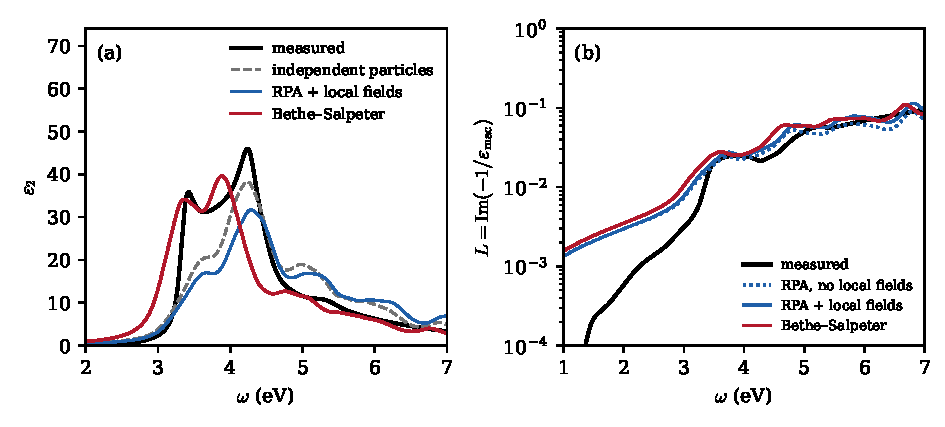
\includegraphics[width=\linewidth]{figures/ch04/fig4_11.pdf}
  \caption{The electron--hole attraction in the optical spectrum of crystalline silicon at $\vect{q} \to 0$, in a model calculation. Band energies and states come from the local empirical pseudopotential of Cohen and Bergstresser~\cite{cohen1966band}, fitted to measured transition energies, as in \cref{fig:4-si-approx}. All curves come from the transition-basis Hamiltonian \cref{eq:4.9-bse} in the Tamm--Dancoff approximation. The basis has 4 valence and 3 conduction bands on a shifted $12^3$ grid of $\vect{k}$ points over the full zone (20{,}736 transitions); both kernels use the 59 shortest reciprocal vectors, and the spectra carry a Lorentzian broadening of \SI{0.15}{eV}. The direct kernel uses the diagonal of the model's static inverse dielectric matrix in the random-phase approximation with local fields, computed with 26 conduction bands; spectra by the Lanczos--Haydock method. Black: measured at \SI{300}{K}~\cite{franta2017temperature}. (a) $\varepsilon_2$: independent particles (dashed gray), the random-phase approximation with local fields, that is, exchange kernel only (blue), and the Bethe--Salpeter equation with both kernels (red). The attraction turns the shoulder near \SI{3.4}{eV} into a peak; the whole spectrum shifts down because the fitted bands already contain part of the excitonic shift. (b) Loss function $L$ on a logarithmic scale for the same three cases (dotted blue: no local fields, which has the independent-particle $\varepsilon_2$). Below about \SI{3}{eV} the model curves are the Lorentzian tails of transitions that start at \SI{3.13}{eV} on this grid, and lie above the measured $L$, which has no such tails.}
  \label{fig:4-bse}
\end{figure}

The attraction restores the lower peak. At \SI{3.42}{eV} independent particles give 15 and local fields 13; with the direct kernel the spectrum has a peak of height 34 at \SI{3.36}{eV}, against the measured 36 at \SI{3.42}{eV}. This peak, however, is not a bound state. The vertical transitions of silicon start near \SI{3.1}{eV}, and the strength comes from many transitions along a region of the zone where conduction and valence bands run nearly parallel, which the attraction mixes coherently. The upper peak moves down to \SI{3.88}{eV}, \SI{0.36}{eV} below the measured \SI{4.24}{eV}, which is the double counting described above. First-principles calculations avoid it by starting from quasiparticle energies of a $GW$ calculation, which contain no excitonic shift. The Bethe--Salpeter spectrum of silicon computed that way by Albrecht and coworkers places both main peaks at the measured energies with the measured ratio of their heights, and overestimates their absolute heights slightly~\cite{albrecht1998ab}. In the model, the static constant rises by 17 percent over the random-phase value with local fields in the same basis of bands. Part of that rise is again the double counting, since $\varepsilon_\infty$ weights each exciton by $1/E_\lambda$, and the ratio is an upper estimate of what the attraction adds to the local-field value of \cref{we:4-siepsinf}.

For dark matter the loss function in panel (b) is the relevant quantity. At \SI{3}{eV} the attraction raises $L$ by 36 percent over the random-phase value with local fields; from 4 to \SI{6}{eV} the two agree within 3.5 percent. The effect is concentrated in the first eV of the absorption, exactly where a slow particle deposits its energy.

At finite $\vect{q}$ the dark-matter rate needs the structure factor rather than $\varepsilon_2$. At $T = 0$ and $\omega > 0$, \cref{eq:4.4-SL} gives $S = (2q^2/e^2)L$, with $L = \Imag(-1/\varepsilon_{\mathrm{mac}}) = \varepsilon_2/|\varepsilon_{\mathrm{mac}}|^2$, and \cref{eq:4.9-eps2} then yields the exciton contribution
\begin{equation}
  S(\vect{q},\omega) = \frac{2\pi g_{\mathrm{deg}}}{\Vol}\sum_\lambda\frac{\bigl|\sum_{cv\vect{k}}A^\lambda_{cv\vect{k}}(\vect{q})\,\rho_{cv}(\vect{k},\vect{q})^*\bigr|^2}{|\varepsilon_{\mathrm{mac}}(\vect{q},\omega)|^2}\,\delta\bigl(\omega - E_\lambda(\vect{q})\bigr) .
  \label{eq:4.9-S}
\end{equation}
Each exciton is a line at $E_\lambda(\vect{q})$ whose weight is its oscillator strength, screened by the factor $1/|\varepsilon_{\mathrm{mac}}|^2$ of \cref{sec:4.4}. The exact statement is $S = (2q^2/e^2)\varepsilon_2/|\varepsilon_{\mathrm{mac}}|^2$, and the line form holds when the line's own contribution to $\varepsilon_{\mathrm{mac}}$ near its energy is small against the background, whose value then goes into the denominator. A line strong enough to change $\varepsilon_{\mathrm{mac}}$ near its own energy is moved up by the long-range exchange energy, since the pole of $L$ sits at the zero of $\varepsilon_{\mathrm{mac}}$. This is the electronic analog of the splitting between the longitudinal optical (LO) and transverse optical (TO) phonons of a polar crystal, in which the macroscopic field of a longitudinal lattice vibration raises its frequency above that of the transverse one (\cref{sec:5.5}). With the $\vect{G} = 0$ term kept in the kernel, the eigenvalues are these shifted energies and the weights are not divided by $|\varepsilon_{\mathrm{mac}}|^2$ (\cref{eq:D.12-S}). At the momentum transfers of a few keV that dark matter typically deposits, the Coulomb factor $e^2/q^2$ is small and the shift is negligible. Without kernels, \cref{eq:4.9-S} is the independent-particle structure factor \cref{eq:4.2-S0} screened by $1/|\varepsilon_{\mathrm{mac}}|^2$, the random-phase result for the electrons.

For a Wannier--Mott exciton, \cref{eq:4.9-elliott} and \cref{eq:4.9-dispersion} make the lines explicit,
\begin{equation*}
  S(\vect{q},\omega) = 2\pi g_{\mathrm{deg}}\,\frac{|\rho_{cv}(\vect{k}_0,\vect{q})|^2}{|\varepsilon_{\mathrm{mac}}(\vect{q},\omega)|^2}\sum_n\frac{1}{\pi a_x^3n^3}\,\delta\bigl(\omega - E_n(\vect{q})\bigr) ,
\end{equation*}
a weight per unit volume set by the probability $|F_{ns}(0)|^2$ of finding the electron at the hole, times the squared vertex between the two band extrema. In silicon the lowest line follows the indirect threshold of \cref{sec:3.3} at $\vect{q} \approx \vect{k}_{\mathrm{c}}$ and lies \SI{14.7}{meV} below it. As a shift of the threshold this is 1.3 percent of the gap, small for the threshold mass of \cref{sec:3.3}. As a redistribution of weight, however, it matters more: the edge of the zero-phonon response starts with a line, and the continuum above it is enhanced. Light dark matter samples exactly this region, and \cref{sec:10.5} computes the excitonic loss function at finite $\vect{q}$.

\subsection{Levels of approximation}

Each approximation contains the previous one as a limit: $K^{\mathrm{d}} \to 0$ gives local fields, $\bar v \to 0$ the random-phase head, and the head alone at fixed energies the independent particles. What the Bethe--Salpeter equation in this form leaves out are the dynamical screening of the interaction, the coupling of pair creation and annihilation, and every process with a phonon, which \cref{chap:6} adds.

In silicon the approximations of \cref{fig:4-si-approx,fig:4-bse} differ in characteristic ways. The static constant falls with the local fields and rises part of the way back with the adiabatic kernel (\cref{we:4-siepsinf}), and in the model the attraction raises it by 17 percent above the local-field value of 10.22, to about 11.9. The screening factor $1/\varepsilon_\infty^2$ at small $q$ thus varies by up to a third across the hierarchy. At the lower absorption peak the spread is a factor of more than two, 13 to 34, and the loss function at \SI{3}{eV} changes by a third between the adiabatic kernel and the Bethe--Salpeter equation alone. Above about \SI{4}{eV}, which holds most of the f-sum, the approximations agree within the accuracy of the bands. As in \cref{sec:4.6}, the spread is an estimate, not a bound. Light dark matter samples the first eV above the gap; for it the attraction is the leading correction, and the Bethe--Salpeter result is the reference against which the cheaper approximations are judged.

\section*{Summary}

A weak field that couples to an operator $O_b$ of a target in equilibrium changes the average of any other operator $O_a$ through the retarded commutator, the Kubo formula $R_{ab}(\vect{q},t) = -(\ii/\Vol)\Theta(t)\langle[O_a(\vect{q},t)^\dagger, O_b(\vect{q},0)]\rangle$ (\cref{sec:4.1}). It holds for any Hamiltonian and at any temperature. Its Lehmann representation has resonant and antiresonant poles at the excitation energies, its imaginary part is the power the target absorbs, and causality makes it analytic in the upper half of the frequency plane. Resonances, such as the plasmon and the quasiparticles, are poles continued below the real axis.

The rate of a dark-matter particle that couples through several operators is an integral over $\vect{q}$ of $\sum_{ab}\tilde V_a^*\tilde V_bS_{ab}(\vect{q},\omega_{\vect{q}})$, with the dynamic structure factor $S_{ab}$ the Fourier transform of an equilibrium correlation function (\cref{sec:4.2}). For the density it is the transform of the Van Hove function, the probability of finding an electron at $\vect{r}$ at time $t$ given one at the origin at time zero. The fluctuation--dissipation theorem, $(1 - \ee^{-\beta\omega})S = -2\Imag R$ on the diagonal, ties the rate to the response, and $S_{ab}$ is a positive semidefinite matrix at every $(\vect{q},\omega)$, so that every rate is positive and every interference is bounded. Without interactions $S$ is the sum over one-electron transitions of \cref{sec:2.5}.

Exact constraints on any computed response follow from causality and from commutators (\cref{sec:4.3}). The Kramers--Kronig relations rebuild the real part from the imaginary one, and the moments of $S$ are equal-time commutators. The first is the f-sum rule, $\int\omega S$ fixed by the density and the mass whatever the interactions, which defines the plasma frequency, \SI{16.6}{eV} for the valence electrons of silicon. The oscillator strengths of an atom obey the Thomas--Reiche--Kuhn rule, a check on tables and on ionization form factors.

The long-range Coulomb interaction is separated once and for all by the dielectric function (\cref{sec:4.4}). The response to the total potential is the proper response $\tilde R$, $\varepsilon = 1 - v_{\mathrm{C}}\tilde R$ and $\varepsilon^{-1} = 1 + v_{\mathrm{C}}R$, and in a crystal both are matrices in the reciprocal-lattice vectors whose inverse defines the macroscopic $\varepsilon_{\mathrm{mac}} = 1/(\varepsilon^{-1})_{\vect{0}\vect{0}}$. The fluctuation--dissipation theorem then writes the structure factor as the loss function, $S = (2q^2/e^2)L/(1 - \ee^{-\beta\omega})$ with $L = \Imag[-(\varepsilon^{-1})_{\vect{0}\vect{0}}]$, so that measured optical and energy-loss spectra enter the rate directly. Silicon has $\varepsilon_\infty = 11.7$, absorption peaks near 3.4 and \SI{4.2}{eV}, and a loss peak of height 4.5 at \SI{16.4}{eV}. Its static screening is metallic at a few keV and insulating below about \SI{1}{keV}. The f-sum and inverse-moment rules fix the main loss peak, but not the low-energy side of $L$ that slow particles, and dark matter, sample.

The homogeneous electron gas is the one system whose response is known in closed form (\cref{sec:4.5}). The Lindhard function is its independent-particle bubble, the random-phase approximation screens it, and at long wavelength the gas oscillates collectively at $\omega_p$ with a dispersion rising as $q^2$, until the plasmon meets the pair continuum at $q_{\mathrm{c}} = \SI{2.60}{keV}$ and decays. A dark-matter particle reaches the plasmon energy only at \SI{6.26}{keV}, beyond $q_{\mathrm{c}}$, and the plasmon is kinematically out of reach. The static Lindhard screening at the typical momentum transfer $q_0$ is $\varepsilon = 2.10$. Mermin's relaxation-time form adds damping without destroying electrons.

In a crystal the bubble becomes the Adler--Wiser matrix of Bloch states (\cref{sec:4.6}). The random-phase approximation with only the head leaves the absorption spectrum unchanged and screens the loss function. The full matrix adds local fields, the microscopic Hartree fields of the induced charge, and time-dependent density-functional theory adds an exchange--correlation kernel. In silicon the local fields lower $\varepsilon_\infty$ by about a tenth, and the adiabatic local-density kernel restores part of it (\cref{we:4-siepsinf}). None of these approximations gives the lower absorption peak. Their spread is the many-body part of the uncertainty of a computed loss function, small for heavier dark matter and leading for light dark matter near the gap.

Green's functions describe one added electron or hole (\cref{sec:4.7}). The spectral function is positive and normalized, the Dyson equation defines the self-energy $\Sigma$, and the poles of the Green's function near the real axis are quasiparticles with energy $E_{\mathrm{qp}}$, residue $z_{\mathrm{qp}}$ and width $\varGamma_{\mathrm{qp}}$. In imaginary time the thermal weight and the time evolution combine into one exponential, so that a single perturbation series serves both, and the analytic continuation from the Matsubara frequencies returns the retarded functions. The quasiparticle correction to Kohn--Sham energies repairs the gap, \SI{0.602}{eV} with PBE against the measured \SI{1.17}{eV} in silicon.

Feynman diagrams organize those series (\cref{sec:4.8}). Wick's theorem reduces every term to products of free propagators, and the Feynman rules turn each diagram into an integral. The random-phase approximation is the chain of bubbles, the proper response the diagrams that one Coulomb line cannot cut, and the screened interaction $W^{\mathrm{scr}} = \varepsilon^{-1}v_{\mathrm{C}}$ replaces the bare one in the $GW$ self-energy. The width of a hot electron is then a dark-matter-like rate with the Coulomb potential in place of $\tilde V$, and the cutting rule shows that every selection of diagrams has a golden-rule reading, $-2\Imag R = (1 - \ee^{-\beta\omega})S$.

The attraction between an excited electron and its hole is the last correction (\cref{sec:4.9}). Summing the ladder diagrams with a statically screened interaction gives the Bethe--Salpeter equation, an eigenvalue problem in the space of transitions with a repulsive exchange kernel, the local fields, and an attractive direct kernel from $W^{\mathrm{scr}}$. Near a band extremum it reduces to hydrogen with the reduced mass $\mu_x$ and the coupling $\alpha/\varepsilon_\infty$, with binding $E_x^b = \mu_x\alpha^2/(2\varepsilon_\infty^2)$. In silicon the measured binding, \SI{14.7}{meV}, is not a prediction of the formula: it fixes $\mu_x = 0.15\,m_e$ and with it a radius of \SI{4.2}{nm}. In GaAs, where the ions screen as well and $\varepsilon_0$ replaces $\varepsilon_\infty$, the formula gives \SI{3.7}{meV} against the measured \SI{4.2}{meV}. Excitons enter $\varepsilon_2$ and the structure factor through coherent oscillator strengths, which move weight toward the gap, and as lines that follow the threshold at finite $\vect{q}$ with the center-of-mass dispersion of the pair. In the model calculation for silicon the attraction restores the lower absorption peak, raises $\varepsilon_\infty$ toward the measured value and the loss function at \SI{3}{eV} by a third; the spread across the completed hierarchy is the many-body uncertainty a computed loss function can quote.

Throughout, the nuclei were held fixed. They move, and their motion adds a second set of excitations, phonons, with energies of tens of meV. It also adds a second contribution to screening in polar crystals and a coupling between electrons and the lattice. \Cref{chap:5} builds the lattice dynamics on which all three rest.
